\documentclass[11pt]{beamer}
\setbeamertemplate{navigation symbols}{}
 \setbeamercovered{transparent}
\usepackage{listings}
%\usetheme{Copenhagen}
\usetheme{Singapore}
%\usetheme{Madrid}
%\usetheme{Hannover}
%\usetheme{boxes}
%\usetheme{Boadilla}
\usefonttheme[onlymath]{serif}
\usecolortheme{beaver}
\usepackage{textpos}
\usepackage{fancyvrb}
\usepackage{xcolor}
\usepackage{multicol}
\usepackage{lipsum}
\parskip 1ex

\newcommand\FontAcolumn{\fontsize{6}{7.2}\selectfont}
\newcommand\FontBcolumn{\fontsize{8}{7.2}\selectfont}
\newcommand\FontCcolumn{\fontsize{10}{7.2}\selectfont}
\newcommand\FontDcolumn{\fontsize{11}{7.2}\selectfont}

\definecolor{gray97}{gray}{.97}
\definecolor{gray75}{gray}{.75}
\definecolor{gray75}{gray}{.45}

\lstdefinestyle{Fortran}{language=[90]Fortran}

\newcommand\FortranStyle
{
\lstset{
frame=Ltb,
framerule=0pt,
columns=fullflexible,
aboveskip=0.5cm,
framextopmargin=3pt,
framexbottommargin=3pt,
framexleftmargin=0.4cm,
framesep=0pt,
rulesep=.4pt,
backgroundcolor=\color{gray97},
rulesepcolor=\color{black},
stringstyle=\ttfamily,
showstringspaces=false,
basicstyle=\ttfamily,
commentstyle=\color{green},
keywordstyle=\color{red},
numbers=left,
numbersep=15pt,
numberstyle=\tiny,
numberfirstline=false,
breaklines=true,
 tabsize=2,
 extendedchars=true,
keepspaces,
}
}

\newcommand\FortranStyleA
{
\lstset{
frame=Ltb,
framerule=0pt,
columns=fullflexible,
aboveskip=0.5cm,
framextopmargin=3pt,
framexbottommargin=3pt,
framexleftmargin=0.4cm,
framesep=0pt,
rulesep=.4pt,
backgroundcolor=\color{gray97},
rulesepcolor=\color{black},
stringstyle=\ttfamily,
showstringspaces=false,
basicstyle=\ttfamily,
commentstyle=\color{green},
keywordstyle=\color{red},
numbersep=15pt,
numberstyle=\tiny,
numberfirstline=false,
breaklines=true,
 tabsize=2,
 extendedchars=true,
keepspaces,
}
}

\newcommand\tab[1][1cm]{\hspace*{#1}}
\newcommand{\light}[1]{\textcolor{lightgray}{#1}}
    
\def\signed #1{{\leavevmode\unskip\nobreak\hfil\penalty50\hskip2em
  \hbox{}\nobreak\hfil(#1)%
  \parfillskip=0pt \finalhyphendemerits=0 \endgraf}}

\newsavebox\mybox
\newenvironment{aquote}[1]
  {\savebox\mybox{#1}\begin{quote}}
  {\signed{\usebox\mybox}\end{quote}}
  
% items enclosed in square brackets are optional; explanation below
\title{Array Concepts}
%\subtitle{Introduction}
\author{Carlos Cruz\\
Jules Kouatchou\\
Bruce Van Aartsen}
\institute{
  NASA GSFC Code 606 (ASTG)\\
  Greenbelt, Maryland 20771\\[1ex]
%  \texttt{carlos.a.cruz@nasa.gov}
}
\date{October 24, 2018}

\begin{document}

% --- Title page ---
\begin{frame}[plain]
  \titlepage
\end{frame}

\logo{%
  
\includegraphics[width=1cm,height=1cm,keepaspectratio]{../../shared/nasa-ball.png}%
  \hspace{\dimexpr\paperwidth-2cm-5pt}%
  
\includegraphics[width=1cm,height=1cm,keepaspectratio]{../../shared/ssai-logo.png}%
}

% --- Slide

\begin{frame}[fragile]
\frametitle{Array Terminology}

\begin{columns}
  \begin{column}{0.5\textwidth}
  \FortranStyle
    \FontBcolumn
\begin{lstlisting}[style=Fortran]
    REAL, DIMENSION(15)       :: A
    REAL, DIMENSION(-4:0,0:2) :: B
    REAL :: C(5,3), D(0:4,0:2) 
\end{lstlisting}
\end{column}

  \begin{column}{0.4\textwidth}
  \FontBcolumn
 \begin{itemize}
 \item \emph{rank} : number of dimensions
 \item \emph{bounds} : upper and  lower limits of indices
\item \emph{extent} : number of elements in dimensions
\item \emph{size} : total number of elements
\item \emph{shape} : rank and extents
\item \emph{conformable} : same shape, B and C and D
 \end{itemize}
 \end{column}
\end{columns}
\bigskip
 
\end{frame}

% --- Slide

\begin{frame}{Array visualization}


\begin{figure}[t]
\centering
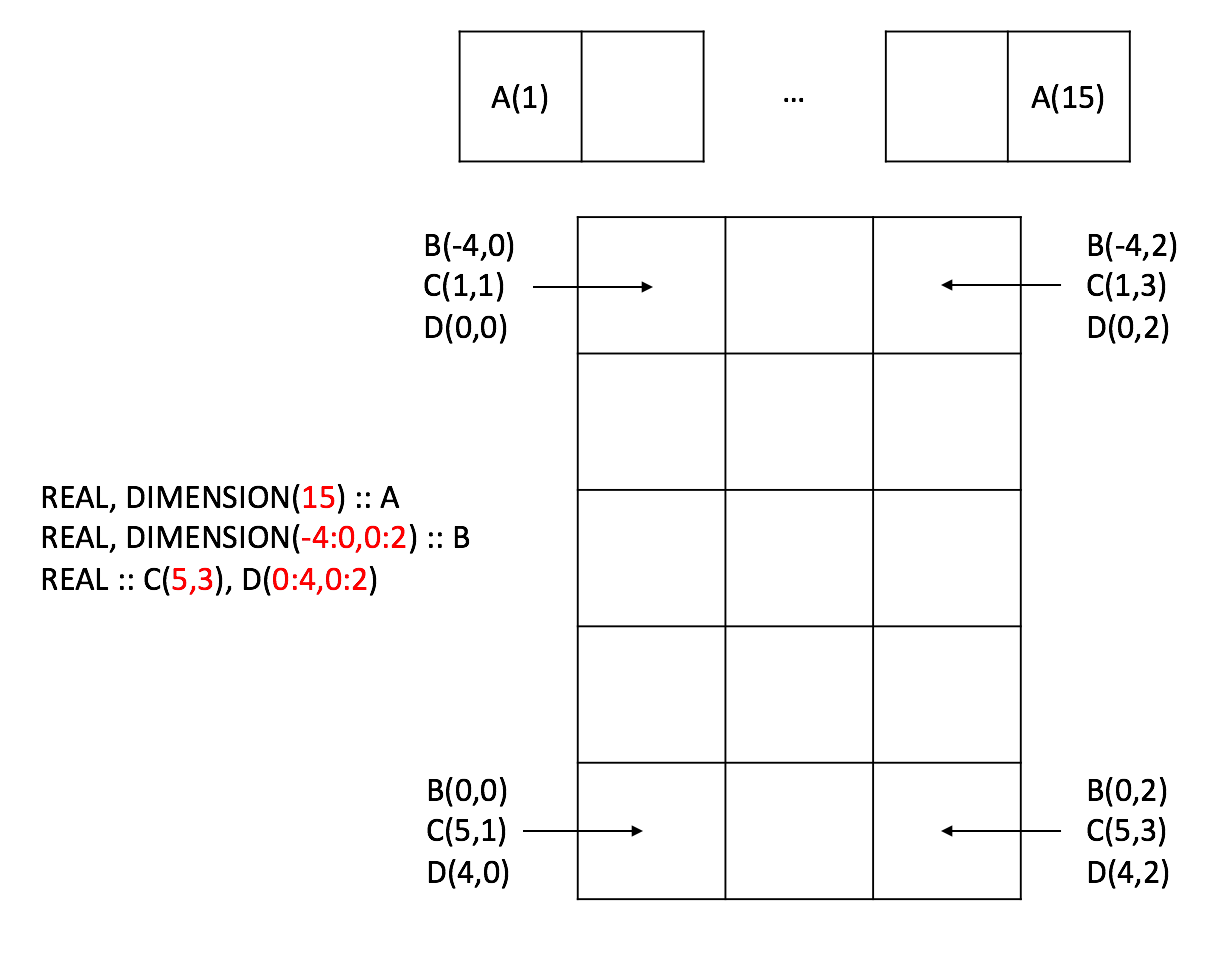
\includegraphics[scale=.4]{array_vis2.png}
\end{figure}
  

\end{frame}


% --- Slide

\begin{frame}[fragile]
\frametitle{Array Declarations}

Literals and constants can be used in array declarations, 
  \FortranStyle
\begin{lstlisting}[style=Fortran]
    REAL, DIMENSION(100)       :: A
    REAL, DIMENSION(10,10)     :: B
    REAL, DIMENSION(-10:-1)    :: X
    INTEGER, PARAMETER :: lda = 5
    REAL, DIMENSION(0:lda-1)   :: Y
    REAL, DIMENSION(1+lda*lda,10) :: Z
\end{lstlisting}

\begin{itemize}
\item default lower bound is 1,
\item bounds can begin and end anywhere,
\item arrays can be zero-sized
 \end{itemize}
\bigskip
 
\end{frame}

% --- Slide

\begin{frame}[fragile]
\frametitle{Array Syntax}

Using the earlier declarations, references can be made to:

\begin{itemize}
\item whole arrays (conformable)
\begin{itemize}
\item A = 0 sets whole array A to zero
\item B = C + 1 adds one to all elements, of C and then assigns each element to the corresponding element of B
 \end{itemize}

\item elements
\begin{itemize}
\item A(1) = 0.0 sets one element to zero
\item B = A(3) + C(5,1) sets whole array B to the sum of two elements
 \end{itemize}

\item array sections
\begin{itemize}
\item A(2:6) = 0 sets section of A to zero
\item B(-1:0,1:2) = C(1:2,2:3) + 1 adds one to the subsection of C and assigns to the subsection of B
 \end{itemize}
 \end{itemize}
\bigskip
 
\end{frame}

% --- Slide

\begin{frame}[fragile]
\frametitle{Array Expressions}

Arrays can be treated like a single variable in that:
\begin{itemize}
\item can use intrinsic operators between conformable arrays (or sections)
\begin{itemize}
\item B = C * D - B**2
 \end{itemize}

\item elemental intrinsic functions can be used
\begin{itemize}
\item B = sin(C) + cos(D)
 \end{itemize}

 \end{itemize}
\bigskip
 
\end{frame}


% --- Slide

\begin{frame}[fragile]
\frametitle{Array Expressions}

\footnotesize{
An array can be subscripted by a \emph{subscript-triplet} giving rise to a sub-array of the original. The general form is: \\
\quad \quad \emph{(start:end:stride)} \\

the section starts at \emph{start} and ends at ot before \emph{end}.\emph{stride}  is the increment by which the locations are selected. \\
\emph{start, end, stride} must all be scalar integer expressions. Thus, these are all valid:
  \FortranStyle
 \begin{lstlisting}[style=Fortran]
   A(m:m) = 0     ! m to m, 1 element array
   A(m:n:k) = 0   ! m to n step k
   A(8:3:-1) = 0  ! 8 to 3 backwards
   A(8:3) = 2     ! step 1 => zero size
   A(M::4) = 1    ! default UPB, step 4
   A(::2) = 1.0   ! default LWB and UPB
   A(m**2:n*k/3) = 1.0
   \end{lstlisting}
}
\end{frame}


% --- Slide

\begin{frame}[fragile]
\frametitle{Array Inquiry}

\footnotesize{
Consider the declaration:
 \begin{lstlisting}[style=Fortran]
 REAL, DIMENSION(-10:10,23,14:28) :: A
 \end{lstlisting}
 Then:
\begin{itemize}
\item LBOUND(SOURCE[,DIM]) -- lower bounds of an array (or bound in an optionally specified dimension).
\begin{itemize}
\item LBOUND(A) is (/-10,1,14/) (array).
\item LBOUND(A,1) is -10 (scalar)
 \end{itemize}
 \item UBOUND(SOURCE[,DIM]) -- upper bounds of an array (or bound in an optionally specified dimension).
\item SHAPE(SOURCE) -- shape of an array.
\begin{itemize}
\item SHAPE(A) is (/21,23,15/) (array).
\item SHAPE((/4/)) is (/1/) (array)
 \end{itemize}
 
 \item SIZE(SOURCE[,DIM]) -- total number of array elements (in an optionally specified dimension).
\begin{itemize}
\item SIZE(A,1) is 21.
\item SIZE(A) is 7245
 \end{itemize}
\item ALLOCATED(SOURCE) -- array allocation status
 \end{itemize}
}

\end{frame}

% --- Slide
\begin{frame}[fragile]
\frametitle{Array Constructors}

\footnotesize{
Used to give arrays or sections of arrays specific values. For example,
  \FortranStyle
 \begin{lstlisting}[style=Fortran]
    IMPLICIT NONE
    INTEGER                        :: i
    INTEGER, DIMENSION(10)         :: ints
    CHARACTER(len=5), DIMENSION(3) :: colours
    REAL, DIMENSION(4)             :: heights
    heights = (/5.10, 5.6, 4.0, 3.6/)
    colours = (/'RED  ','GREEN','BLUE '/)
    ! note padding so strings are 5 chars
    ints    = (/ 100, (i, i=1,8), 100 /)
     \end{lstlisting}
 Then:
\begin{itemize}
\item constructors and array sections must conform.
\item must be 1D.
\item for higher rank arrays use RESHAPE intrinsic
 \end{itemize}
}

\end{frame}

% --- Slide
\begin{frame}[fragile]
\frametitle{RESHAPE}

\footnotesize{
 RESHAPE is a general intrinsic function which delivers an array of a specific shape: 
  \begin{lstlisting}[style=Fortran]
RESHAPE(SOURCE, SHAPE)
   \end{lstlisting}
 e.g.:
   \begin{lstlisting}[style=Fortran]
A = RESHAPE((/1,2,3,4/),(/2,2/))
   \end{lstlisting}
A is filled in array element order and looks like: 

\begin{Verbatim}
    1    3
    2    4
 \end{Verbatim}
}

\end{frame}

% --- Slide
\begin{frame}[fragile]
\frametitle{Array Constructors in Initialization Statements}

\footnotesize{
Named array constants can be created
  \FortranStyle
 \begin{lstlisting}[style=Fortran]
    INTEGER, DIMENSION(3), PARAMETER :: &
        Unit_vec = (/1,1,1/)
    CHARACTER(LEN=*), DIMENSION(3),  PARAMETER :: &
        lights =  (/'RED  ','BLUE ','GREEN'/)
    REAL, DIMENSION(3,3), PARAMETER :: &
        unit_matrix = RESHAPE( &
        (/1,0,0,0,1,0,0,0,1/),(/3,3/))
 \end{lstlisting}
 In the second statement all strings must be same length. 
}

\end{frame}

% --- Slide
\begin{frame}[fragile]
\frametitle{Allocatable Arrays}

\footnotesize{
Fortran allows arrays to be created on-the-fly; these are known as \emph{deferred-shape} arrays and use dynamic heap storage. \\
Deferred-shape arrays are
\begin{itemize}
\item declared like explicit-shape arrays but without the extents and with the ALLOCATABLE attribute.
\begin{itemize}
\item INTEGER, DIMENSION(:), ALLOCATABLE :: ages
\item REAL, DIMENSION(:,:), ALLOCATABLE :: speed
 \end{itemize}
 \item given a size in an ALLOCATE statement which assigns an area of memory to the object.
\begin{itemize}
\item ALLOCATE(ages(1:10), STAT=ierr)
\item ALLOCATE(speed(-lwb:upb,-50:0),STAT=ierr)
 \end{itemize}
\item the optional STAT= field reports on the success of the storage request. If the INTEGER variable ierr is zero the request was successful otherwise it failed. 
 \end{itemize}
}

\end{frame}

% --- Slide
\begin{frame}[fragile]
\frametitle{Deallocating Arrays}

\footnotesize{
Heap storage can be reclaimed using the DEALLOCATE statement:
 \begin{lstlisting}[style=Fortran]
IF (ALLOCATED(ages)) DEALLOCATE(ages,STAT=ierr)
 \end{lstlisting}

\begin{itemize}
\item it is an error to deallocate an array without the ALLOCATE attribute or one that has not been previously allocated space.
\item there is an intrinsic function, ALLOCATED, which returns a scalar LOGICAL values reporting on the status of an array. 
\item the STAT= field is optional but its use is recommended
\item if a procedure containing an allocatable array which does not have the SAVE attribute is exited without the array being DEALLOCATE d then this storage becomes inaccessible
 \end{itemize}
}

\end{frame}


% --- Slide
\begin{frame}[fragile]
\frametitle{Masked Array Assignment - Where Statement}

\footnotesize{
This is achieved using WHERE
 \begin{lstlisting}[style=Fortran]
WHERE (I /= 0) A = B/I
 \end{lstlisting}
the LHS of the assignment must be array valued and the mask, (the logical expression,) and the RHS of the assignment must all conform. \\
For example, if 
\[
B = 
 \begin{pmatrix}
  1.0 & 2.0  \\
  3.0 & 4.0  \\
 \end{pmatrix}
 \]
and
\[
I = 
 \begin{pmatrix}
  2 & 0  \\
  0 & 2  \\
 \end{pmatrix}
 \]
then
\[
A = 
 \begin{pmatrix}
  0.5 & -  \\
  - & 2.0  \\
 \end{pmatrix}
 \]
Only the elements, corresponding to the non-zero elements of I, have been assigned to.
}

\end{frame}

% --- Slide
\begin{frame}[fragile]
\frametitle{Where Construct}

\footnotesize{
There is a block form of masked assignment
  \FortranStyle
\begin{lstlisting}[style=Fortran]
 WHERE(A > 0.0)
     B = LOG(A)
     C = SQRT(A)
  ELSEWHERE
     B = 0.0
  ENDWHERE
\end{lstlisting}
\begin{itemize}
\item the mask must conform to the RHS of each assignment; A, B and C must conform.
\item WHERE ... END WHERE is not a control construct and cannot currently be nested. 
\item the STAT= field is optional but its use is recommended
\item the execution sequence is as follows: evaluate the mask, execute the WHERE block (in full) then execute the ELSEWHERE block
\item the separate assignment statements are executed sequentially but the individual elemental assignments within each statement are (conceptually) executed in parallel
 \end{itemize}
}

\end{frame}

% --- Slide
\begin{frame}[fragile]
\frametitle{Vector-valued subscripts}

\footnotesize{
A 1D array can be used to subscript an array in a dimension. Consider
\begin{lstlisting}[style=Fortran]
    INTEGER, DIMENSION(5) :: V = (/1,4,8,12,10/)
    INTEGER, DIMENSION(3) :: W = (/1,2,2/)
 \end{lstlisting}
\begin{itemize}
\item A(V) is A(1), A(4), A(8), A(12), and A(10).
\item the following are valid assignments:
\begin{lstlisting}[style=Fortran]
    A(V) = 3.5
    C(1:3,1) = A(W)
 \end{lstlisting}
\item it would be invalid to assign values to A(W) as A(2) is referred to twice
\item only 1D vector subscripts are allowed, for example
\begin{lstlisting}[style=Fortran]
    A(1) = SUM(C(V,W))
 \end{lstlisting}
 \end{itemize}
}

\end{frame}


% --- Slide

\begin{frame}[fragile]
\frametitle{Exercise}

Consider the following declaration:
  \FortranStyle
 \begin{lstlisting}[style=Fortran]
 integer, parameter :: MONTHS_PER_YEAR  =  12
 INTEGER, parameter :: &
 DAYS_PER_MONTH (MONTHS_PER_YEAR) = (/  &
 31, 28, 31, 30, 31, 30, 31, 31, 30, 31, 30, 31  /)
 \end{lstlisting}
\begin{itemize}
\item What is the output of DAYS\_PER\_MONTH(1:12:2)?
\item Extract from DAYS\_PER\_MONTH all the months with 30 days and assign the result to a variable. Should be a one-liner?
 \end{itemize}

\end{frame}

\end{document}
